\documentclass[12pt,border=5pt]{standalone}
\usepackage[T1]{fontenc}
\usepackage{lmodern,amsmath,amssymb,bm,tikz}
\usetikzlibrary{arrows.meta,positioning,calc,shapes.geometric,fit,matrix}
\newcommand{\RR}{\mathbb R}
\newcommand{\norm}[1]{\left\lVert#1\right\rVert}
\DeclareMathOperator{\col}{col}
\DeclareMathOperator{\diag}{diag}
\definecolor{plantblue}{HTML}{247BA0}
\definecolor{plantteal}{HTML}{16856B}
\definecolor{plantorange}{HTML}{D97425}
\definecolor{plantpurple}{HTML}{7954A1}
\begin{document}
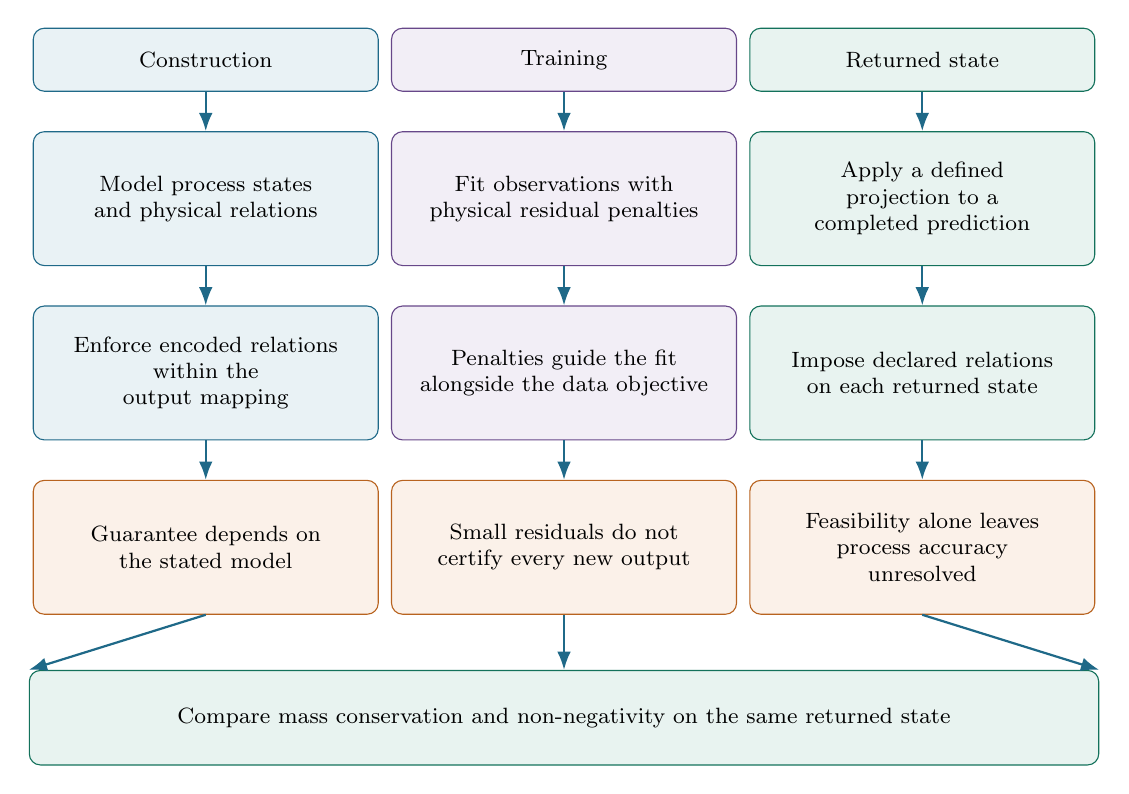
\begin{tikzpicture}[>=Latex,node distance=5mm,
heading/.style={draw=plantblue!85!black,rounded corners,fill=plantblue!8,text width=4.1cm,minimum height=8mm,align=center,font=\footnotesize,inner sep=4pt},
block/.style={heading,fill=white,minimum height=17mm},
limit/.style={block,fill=plantteal!9},
flow/.style={->,thick,draw=plantblue!85!black}]
\node[heading,draw=plantblue!85!black,fill=plantblue!10] (lh) at (-4.55,0) {Construction};
\node[heading,draw=plantpurple!85!black,fill=plantpurple!10] (mh) at (0,0) {Training};
\node[heading,draw=plantteal!85!black,fill=plantteal!10] (rh) at (4.55,0) {Returned state};
\node[block,below=of lh,draw=plantblue!85!black,fill=plantblue!10] (l1) {Model process states\\and physical relations};
\node[block,below=of mh,draw=plantpurple!85!black,fill=plantpurple!10] (m1) {Fit observations with\\physical residual penalties};
\node[block,below=of rh,draw=plantteal!85!black,fill=plantteal!10] (r1) {Apply a defined\\projection to a\\completed prediction};
\node[block,below=of l1,draw=plantblue!85!black,fill=plantblue!10] (l2) {Enforce encoded relations\\within the\\output mapping};
\node[block,below=of m1,draw=plantpurple!85!black,fill=plantpurple!10] (m2) {Penalties guide the fit\\alongside the data objective};
\node[block,below=of r1,draw=plantteal!85!black,fill=plantteal!10] (r2) {Impose declared relations\\on each returned state};
\node[limit,below=of l2,draw=plantorange!85!black,fill=plantorange!10] (l3) {Guarantee depends on\\the stated model};
\node[limit,below=of m2,draw=plantorange!85!black,fill=plantorange!10] (m3) {Small residuals do not\\certify every new output};
\node[limit,below=of r2,draw=plantorange!85!black,fill=plantorange!10] (r3) {Feasibility alone leaves\\process accuracy\\unresolved};
\node[heading,text width=13.3cm,minimum height=12mm,below=7mm of m3,draw=plantteal!85!black,fill=plantteal!10] (common)
{Compare mass conservation and non-negativity on the same returned state};
\draw[flow] (lh)--(l1); \draw[flow] (l1)--(l2); \draw[flow] (l2)--(l3);
\draw[flow] (mh)--(m1); \draw[flow] (m1)--(m2); \draw[flow] (m2)--(m3);
\draw[flow] (rh)--(r1); \draw[flow] (r1)--(r2); \draw[flow] (r2)--(r3);
\draw[flow] (l3.south)--(common.north west);
\draw[flow] (m3.south)--(common.north);
\draw[flow] (r3.south)--(common.north east);
\end{tikzpicture}

\end{document}
